
\documentclass[12pt]{article}
\usepackage{geometry}
 \geometry{letterpaper,left=25mm,top=25mm,right=25mm}
\usepackage[utf8]{inputenc}
\usepackage[spanish]{babel} %Poner algunas palabras reservadas en español
\usepackage{authblk} %Poner instituto en la portada
%Paquetes para símbolos matematicos
\usepackage{amsmath}
\usepackage{mathtools}
\usepackage{amsthm}
\usepackage{amssymb}
\usepackage{bbm}
\usepackage[]{algorithm2e} %Paquete para algoritmos
\usepackage{enumerate}
%Paquete para imagenes
\usepackage{graphicx}
\graphicspath{{img/}}
%Paquete para teoremas
\newtheorem*{thm}{Teorema}
%Quitar la sangria
\setlength{\parindent}{0cm}

\title{Tarea 2}
\author{Fernando Márquez Pérez \\ Juan Antonio Jasso Oviedo \\ Emiliano Dom\'inguez Cruz}
\date{04/10/2019}
\affil{Facultad de Ciencias\\UNAM}

\begin{document}
\begin{titlepage}
    \maketitle
\end{titlepage}

%EJERCICIO 1 ----------------------------------------------------------------------------------
1. Determine si las siguientes funciones son continuas en \(x_0\).

\begin{enumerate}[\hspace{9px} a)]
    %EJERCICIO A    
    \item
    \( f(x)=
    \begin{cases}
        \sqrt{x^2-1}\text{, si} \ x \geq 1\\
        x^2-2x+1\text{, si} \ x \in [0,1]
    \end{cases}
    \)
    en $x_0 = 1$\\

        Primero obtenemos $f(x_0)$: \quad \(f(1) = (1)^2-2(1)+1 = 1-2+1 = 0\)

        Luego buscamos el l\'imite por la izquiera y por la derecha:\\

        \(\displaystyle\lim_{x \to 1^+}f(x)=\lim_{x \to 1^+}\sqrt{x^2-1} = \sqrt{1^2-1} = \sqrt{0} = 0\)

        \(\displaystyle\lim_{x \to 1^-}f(x)=\lim_{x \to 1^-}x^2-2x+1 = \lim_{x \to 1^-}x^2 -\lim_{x \to 1^-}2x + \lim_{x \to 1}1 = 1^1-2(1)+1=0\)\\

        Como \(\displaystyle\lim_{x \to 1^+}f(x)=\lim_{x \to 1^-}f(x)=f(1)\), \textbf{la funci\'on es continua en $x_0=1$.}\\

    %EJERCICIO B        
    \item
    \( h(x)=
    \begin{cases}
        \frac{|x|}{x}\text{, si} \ x \neq 0\\
        1\text{, si} \ x=0\\
    \end{cases}
    \)
    en $x_0=0$\\

        Primero obtenemos $h(x_0)$: \quad \(h(0) = 1)\)

        Luego buscamos el l\'imite por la izquierda y por la derecha:\\

        \(\displaystyle\lim_{x \to 0^+}h(x)=\lim_{x \to 0^+}\frac{|x|}{x}\)

        Como es el l\'imite por la derecha, consideramos a todos los $x : x>0$. Como $x>0$, $|x|=x$ (Por la definición de valor absoluto), entonces podemos reescribir el l\'imite como:

        \(\displaystyle\lim_{x \to 0^+}h(x)=\lim_{x \to 0^+}\frac{x}{x}=\lim_{x \to 0^+}1=1\)\\

        \(\displaystyle\lim_{x \to 0^-}h(x)=\lim_{x \to 0^-}\frac{|x|}{x}\)

        Como es el l\'imite por la izquierda, consideramos a todos los $x : x<0$. Como $x<0$, $|x|=-x$ (Por la definición de valor absoluto), entonces podemos reescribir el l\'imite como:

        \(\displaystyle\lim_{x \to 0^+}h(x)=\lim_{x \to 0^+}\frac{-x}{x}=\lim_{x \to 0^+}-1=-1\)\\

        Entonces tenemos que: \quad \(\displaystyle\lim_{x \to 0^+}h(x)\neq\lim_{x \to 0^-}h(x)\)\\

        Por lo tanto, \textbf{la funci\'on no es continua en $x_0=0$}\\

    %EJERCICIO C
    \item
    \( g(x)=
    \begin{cases}
        \sqrt{1-x^2}\text{, si} \ x \in [0,1]\\
        -\sqrt{1-(x-2)^2}\text{, si} \ x \in [1,2]
    \end{cases}
    \)
    en $x_0=1$\\

        Primero obtenemos $f(x_0)$:\\
        
        \(g(1) = \sqrt{1-(1)^2} =  \sqrt{0} = 0\)
        
        \(g(1) = -\sqrt{1-((1)-2)^2} = -\sqrt{1-(-1)^2} = -\sqrt{1-1} = -\sqrt{0} = 0\)\\

        Luego buscamos el l\'imite por la izquierda y por la derecha:\\

        \(\displaystyle\lim_{x \to 1^+}g(x)=\lim_{x \to 1^+}-\sqrt{1-(x-2)^2} = -\sqrt{1-(-1)^2} = -\sqrt{1-1} = -\sqrt{0} = 0\)

        \( \displaystyle\lim_{x \to 1^-}g(x)=\lim_{x \to 1^-}\sqrt{1-(1)^2} = \sqrt{0} = 0\)\\

        Como \(\displaystyle\lim_{x \to 1^+}g(x)=\lim_{x \to 1^-}g(x)=g(1)\), \textbf{la funci\'on es continua en $x_0=1$.}\\

\end{enumerate}

%EJERCICIO 2 ----------------------------------------------------------------------------------
2. Se inyecta un fármaco a un paciente cada 12 horas. En la Fig. 1 se muestra la concentración $c(t)$ del fármaco en el torrente sanguieo después de $t$ horas.
\begin{figure}[h]
    \centering
    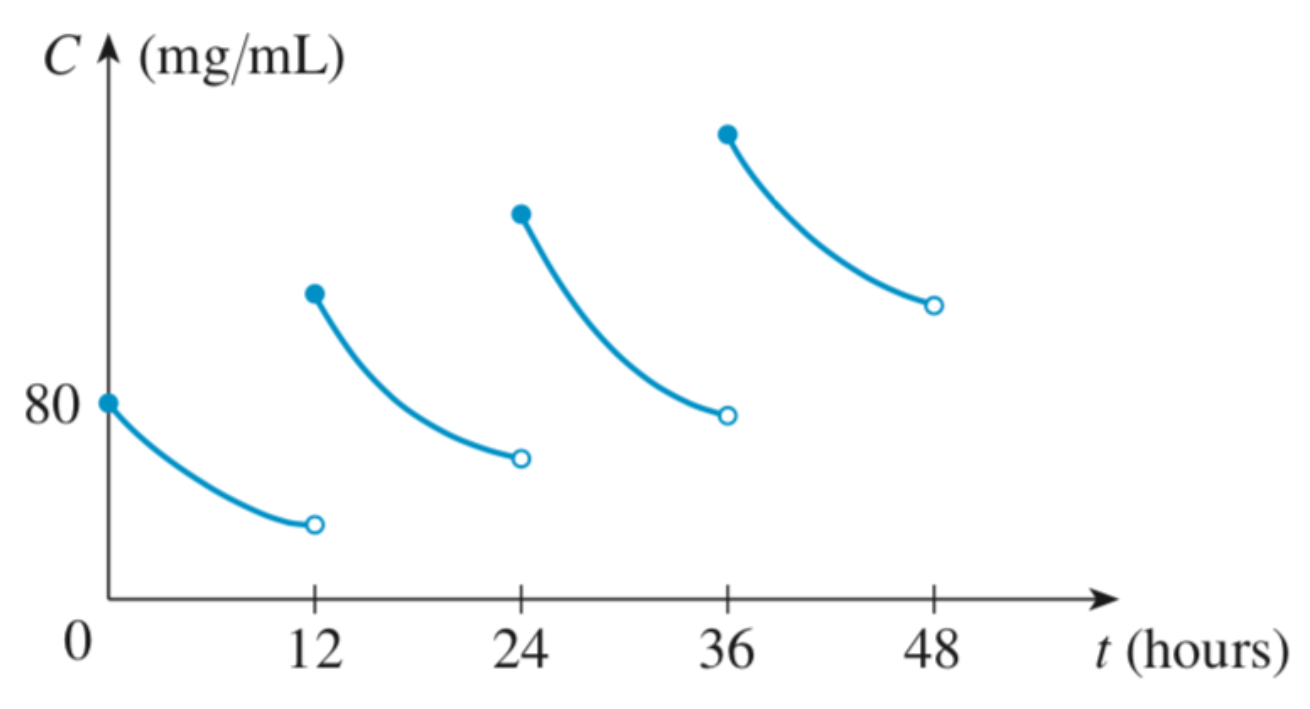
\includegraphics[width=0.5\textwidth]{fig1}
    \caption{Concentraci\'on de f\'armaco}
\end{figure}
\begin{enumerate}[\hspace{9px} a)]
    \item ¿Para qué valores de $t$, $c(t)$ tiene discontinuidades?
    
        Para 12, 24, 36 y 48

    \item ¿Qué tipo de discontinuidades tiene?
    
        Como para todos los puntos $x_i$ enunciados en el inciso pasado, \(\displaystyle\lim_{x \to x_i^+}f(x) \neq \lim_{x \to x_i^-}f(x)\), el l\'imite no existe, por lo que la discontinuidad es irremovible.\\\vspace{\fill}

\end{enumerate}

\bigskip

%EJERCICIO 3 ----------------------------------------------------------------------------------
3. Mostrar que existe algún número $x$, tal que:

\begin{enumerate}[\hspace{9px} a)]
    %EJERCICIO A
    \item \(\sin x = x-1\)\\

        Reescribimos la igualdad como \(\sin(x)-(x-1)=0 \Longrightarrow \sin(x)-x+1=0\)\\

        Como $\sin(x)$ es continua y $x-1$ es un polinomio y todos los polimonios son continuos. Su suma es una función continua. Entonces \(f(x)=\sin(x)-x+1\) es continua en todos los $\mathbbm{R}$.\\

        Para utilizar el TVI, buscamos $f(a)$ y $f(b)$ tal que $f(a)<0<f(b)$.\\

        Proponemos $a=0$ y $b=\pi$
        \[f(0)=\sin(0)-0+1=0-0+1=1\]
        \[f(\pi)=\sin(\pi)-\pi+1=0-\pi+1 \approx -2.1416\]

        Como $f$ es continua en el intervalo $[0,\pi]$ y \(f(0)>0>f(\pi)\), podemos utilizar un derivado del TVI (Parte de un corolario) para decir que: \[\exists \ x_0 \in (0,\pi) : \ f(x_0)=0\]

    %EJERCICIO B
    \item \(x^{179}+\displaystyle\frac{163}{1+x^2+\sin^2 x}=119\)\\

        Reescribimos la igualdad como \(x^{179}+\displaystyle\frac{163}{1+x^2+\sin^2 x}-119=0\)\\

        Como $\sin(x)$ es continua, $\sin^2(x)$ es continua. De igual manera, $x^2$ es continua, por lo que $1+x^2+\sin^2(x)$ es continua.

        \[0<1<1+x^2+\sin^2(x) \quad \text{Porque, por el cuadrado, ambos son positivos $\forall \ x \in \mathbbm{R}$}\]

        Como $1+x^2+\sin^2(x)$ nunca es 0, $\displaystyle\frac{163}{1+x^2+\sin^2(x)}$ es continua en todos los $\mathbbm{R}$. $x^{179}$ también es continua, por lo que \(f(x)=x^{179}+\displaystyle\frac{163}{1+x^2+\sin^2(x)}-119\) \ es continua en todos los $\mathbbm{R}$.\\

        Para utilizar el TVI, buscamos $f(a)$ y $f(b)$ tal que $f(a)<0<f(b)$.\\

        Proponemos $a=-1$ y $b=0$
        \[f(0)=0^{179}+\displaystyle\frac{163}{1+0^2+\sin^2(0)}-119 = 0+\displaystyle\frac{163}{1+0+0}-119 = 163-119 = 44\]
        \begin{multline*}
            f(-1)=(-1)^{179}+\displaystyle\frac{163}{1+(-1)^2+\sin^2(-1)}-119 \approx -1+\displaystyle\frac{163}{1+1+1}-119 \\ \approx -1+\displaystyle\frac{163}{3}-119 \approx -1+54.3-119 \approx -65.7
        \end{multline*}

        Nota: La respuesta correcta es $f(-1)=-59.8$, y difiere de lo obtenido por que $\sin(-1)=-0.84$ y nosotros consideramos $\sin(-1) \approx -1$\\

        Como $f$ es continua en el intervalo $[-1,0]$ y \(f(-1)<0<f(0)\), podemos utilizar el TVI para decir que: \[\exists \ x_0 \in (-1,0) : \ f(x_0)=0\]

    %EJERCICIO C
    \item \(\cos x - \displaystyle\frac{1}{2}=x-1\)\\

        Reescribimos la igualdad como \(\cos(x)-\displaystyle\frac{1}{2}-(x-1)=0 \Longrightarrow \cos(x)+\displaystyle\frac{1}{2}-x=0\).\\

        Como $\cos(x)$ y $x$ son continuos, y la suma de continuos es continua, $f(x)=\cos(x)-x+\displaystyle\frac{1}{2}$ es continua en todos los $\mathbbm{R}$.\\

        Para utilizar el TVI, buscamos $f(a)$ y $f(b)$ tal que $f(a)<0<f(b)$.\\

        Proponemos $a=0$ y $b=\pi$
        \[f(0)=\cos(0)-0+\frac{1}{2} = 1-0+\frac{1}{2} = \frac{3}{2}\]
        \[f(\pi)=\cos(x)-x+\frac{1}{2} = 0-\pi+\frac{1}{2} \approx -2.6\]

        Como $f$ es continua en el intervalo $[0,\pi]$ y \(f(0)>0>f(\pi)\), podemos utilizar un derivado del TVI (Parte de un corolario) para decir que: \[\exists \ x_0 \in (0,\pi) : \ f(x_0)=0\]


    \smallskip
    %EJERCICIO D
    \item \((2x^2-2)^2=-x+1\)\\

    Reescribimos la igualdad como \((2x^2-2)^2-(-x+1)=0 \Longrightarrow (2x^2-2)^2+x-1=0\).\\

    Como $2x^2-2$ y $-x+1$ son polinomios, son continuos. Como la multiplicación de dos continuos es continua, $(2x^2-2)^2$ es continua. Y dado que la suma de dos continuos es continua $f(x)=(2x^2-2)^2+x-1$ es continua en todos los $\mathbbm{R}$.\\

    Para que $f$ cumpla el TVI tiene que existir un $f(x_0)<0$, pero $f$ nunca es menor a 0:

    Observación: Sabemos que $(2x^2-2)^2 \geq 0 \ \forall \ x \in \mathbbm{R}$\\

    Para $x \leq 1$:
    \[x \leq 1 \Rightarrow x-1 \leq 0 \leq (2x^2-2)^2 \Rightarrow x-1 \leq (2x^2-2)^2 \Rightarrow 0 \leq (2x^2-2)^2-(x-1)\]

    Para $x>1$:
    \[x>1 \Rightarrow x-1>0 \Rightarrow x-1+(2x^2-2)^2>0\]

    Pero si proponemos $x_0=1$:

    \[f(1)=(2(1)^2-2)^2+1-1=(2-2)^2+0=0^2+0=0\]

    Obtenemos el $x_0$ que cumple la igualdad.\\

\end{enumerate}

%EJERCICIO 4 ----------------------------------------------------------------------------------
4. Vea si en los siguientes incisos se cumple el teorema de valor intermedio y, en ese caso, calcula un valor intermedio.

\begin{enumerate}[\hspace{9px} a)]
    %EJERCICIO A
    \item \(f(x)=x^3\) en $[-1,1]$\\

        Obtenemos $f(-1)$ y $f(1)$:
        \begin{align*}
            &f(-1) = (-1)^3 = -1  &&f(1) = (1)^3 = 1
        \end{align*}

        Sabemos que $f$ es un polinomio de grado 3 y que todos los polinomios son continuos en $\mathbbm{R}$, por ende, $f$ es continua en $[-1,1]$.\\

        Como $f(-1) < 0 < f(1)$ y $f(x)$ es continua en $[-1,1]$. Podemos usar el \textbf{Teorema del Valor Intermedio} para decir que: \(\exists \ x_0 \in (-1,1) : \ f(x_0)=0\).\\

        Ahora buscamos a $x_0$:
        \begin{equation*}
            f(x_0)=0 \Rightarrow (x_0)^3 = 0 \Rightarrow (x_0)(x_0)(x_0)=0 \Rightarrow x_0=0
        \end{equation*}

        \textbf{$\mathbf{\therefore \ f(x)}$ cumple el Teorema del Valor Intermedio en el intervalo dado. Un valor intermedio es $\mathbf{x_0=0}$.}\\

    %EJERCICIO B
    \item \(g(x)=x^3\) en $[0,2]$\\

        Obtenemos $g(0)$ y $g(2)$:
        \begin{align*}
            &g(0)=(0)^3=0 &&g(2)=(2)^3=8
        \end{align*}

        Estrictamente hablando, $g(x)$ no cumple el \textbf{Teorema del Valor Intermedio} porque \(g(0) < 0 < g(2)\) no es verdad porque $g(0)=0$. Pero es eso se debe a que justo el intervalo toma al $x_0$ que cumple $g(x_0)=0$: $\mathbf{x_0=0}$\\

    %EJERCICIO C
    \item \(h(x)=x^2+4x+4\) en $[0,1]$\\

        Obtenemos $h(0)$ y $h(1)$:
        \begin{align*}
            &h(0)=(0)^2+4(0)+4=4 &&h(1)=(1)^2+4(1)+4=1+4+4=9
        \end{align*}

        Como $h$ es un polinomio, es continua en $[0,1]$.\\

        Tenemos, entonces, que \(h(0) > 0 < h(1)\). Como esto no cumple el \textbf{TVI}, buscamos valores dentro de $[0,1]$ que puedan cumplirlo.\\

        Proponemos el intervalo $\left[\frac{1}{2},1\right] \in [0,1]$\\

        Obtenemos \(h\left(\displaystyle\frac{1}{2}\right)\): \quad \(\left(\displaystyle\frac{1}{2}\right)^2+4\left(\displaystyle\frac{1}{2}\right)+4 = \left(\displaystyle\frac{1}{4}\right)+2+4 = \displaystyle\frac{1}{4}+\displaystyle\frac{24}{4}=\displaystyle\frac{25}{4}\)
        \\

        Como \(h\left(\displaystyle\frac{1}{2}\right) > 0 < h(1)\) podemos concluir que:\\

        \textbf{$h(x)$ NO cumple el Teorema del Valor Intermedio en el intervalo dado.}\\

        Lo que tiene sentido porque si buscamos las raices de $f(x)$ obtendremos:
        \begin{equation*}
            h(x_0) \Rightarrow x_0^2+4x_0+4=0 \Rightarrow (x_0+2)^2=0 \Rightarrow x_0+2=0 \Rightarrow x_0=-2
        \end{equation*}

    %EJERCICIO D
    \item \(k(x)=3x^2-x-1\) en $[-1,1]$\\

        Obtenemos $k(-1)$ y $k(1)$:
        \begin{align*}
            &k(-1)=3(-1)^2-(-1)-1=3(1)+1-1=3 \\
            &k(1)=3(1)^2-1-1=3(1)-1-1=3-2=1
        \end{align*}

        Como $k$ es un polinomio, es continua en $[-1,1]$.\\

        Tenemos, entonces, que \(k(-1) > 0 < k(1)\). Como esto no cumple el \textbf{TVI}, buscamos valores dentro de $[0,1]$ que puedan cumplirlo.\\

        Proponemos el intervalo $[0,1] \in [-1,1]$\\

        Obtenemos $k(0)$: \quad \(3(0)^2-0-1=0-0-1=-1\)\\

        Como tenemos que \(k(0) < 0 < k(1)\) y que $k$ es continua en el intervalo. Podemos usar el \textbf{Teorema del Valor Intermedio} para decir que: \(\exists \ x_0 \in (-1,1) : \ k(x_0)=0\).\\

        Ahora buscamos $x_0$: \quad $3x^2-x-1=0$\\

        Para encontrar $x_0$ cerramos el intervalo:
        \[k\left(\displaystyle\frac{1}{2}\right) = 3\left(\frac{1}{2}\right)^2-\left(\frac{1}{2}\right)-1=\frac{3}{4}-\frac{6}{4}=-\frac{3}{4}\]

        Si proponemos el intervalo $\left[\displaystyle\frac{1}{2},1\right]$ Tenemos que:

        \(k\left(\displaystyle\frac{1}{2}\right) < 0 < k(1) \Longrightarrow -\displaystyle\frac{3}{4} <0<1\).\\

        Como seguimos cumpliendo el TVI. Seguimos cerrando en intervalo:

        \[k\left(\displaystyle\frac{3}{4}\right)=3\left(\frac{3}{4}\right)^2-\left(\frac{3}{4}\right)-1=\frac{27}{16}-\frac{7}{4}=\frac{27}{16}-\frac{28}{16}=-\frac{1}{16}\]

        $-\displaystyle\frac{1}{16}$ es un valor muy cercano a 0. Por lo que podemos decir que $x_0 \approx \displaystyle\frac{3}{4}$

        Lo que tiene sentido porque si obtenemos las raices de $k$ usando la f\'ormula general, tenemos que:

        \(x=\displaystyle\frac{-b\pm \sqrt{b^2-4ac}}{2a}\) \quad Donde $a=3$, $b=-1$ y $c=-1$.

        \begin{align*}
            x&=\frac{-(-1)\pm \sqrt{(-1)^2-4(3)(-1)}}{2(3)}\\
            &=\frac{1\pm \sqrt{1+12}}{6}\\
            &=\frac{1\pm \sqrt{13}}{6}
        \end{align*}
        y \ \(\displaystyle\frac{1+\sqrt{13}}{6} \approx \frac{3}{4}\)\\

        \textbf{$\mathbf{\therefore \ k(x)}$ cumple el Teorema del Valor Intermedio en el intervalo dado. Un valor intermedio es $\mathbf{x_0=\displaystyle\frac{1+\sqrt{13}}{6}}$.}\\

\end{enumerate}

%EJERCICIO 5 ----------------------------------------------------------------------------------
5. Pruebe que las ecuaciones dadas, tienen una raíz en el intervalo que se señala.

\begin{enumerate}[\hspace{9px} a)]
    %EJERCICIO A
    \item \(x^3+7x^2-3x-5=0\) en $[-3.2,0.1]$\\

        Consideramos en intervalo $[-3,0] \in [-3.2,0.1]$. Como $[-3,0] \in [-3.2,0.1]$, si hay un raíz en $[-3,0]$, hay una raíz en $[-3.2,0.1]$.\\

        Obtenemos $f(-3)$ y $f(0)$:
        \[f(-3)=(-3)^3+7(-3)^2-3(-3)-5=-27+7(9)+9-5=-27+63+9-5=40\]
        \[f(0)=0^3+7(0)^2-3(0)-5=0+0-0-5=-5\]

        Como $f$ es un polinomio, es continua en $[-3,0]$. Además tenemos que $f(-3)>0>f(0)$. Por lo que podemos usar un derivado del TVI para decir que: \(\exists \ x_0 \in (-3,0) : \ f(x_0)=0\)\\

        \textbf{ $\therefore \ f$ tiene una raíz en $[-3.2,0.1]$}\\
    %EJERCICIO B
    \item \(x^5-4x^3+x^2-1=0\) en $[-2.1,1.5]$

        Consideramos en intervalo $[-1,0] \in [-2.1,1.5]$. Como $[-1,0] \in [-2.1,1.5]$, si hay un raíz en $[-1,0]$, hay una raíz en $[-2.1,1.5]$.\\

        Obtenemos $f(-1)$ y $f(0)$:
        \[f(-1)=(-1)^5-4(-1)^3+(-1)^2-1=-1+4+1-1=3\]
        \[f(0)=0^5-4(0)^3+0^2-1=0-0+0-1=-1\]

        Como $f$ es un polinomio, es continua en $[-1,0]$. Además tenemos que $f(-1)>0>f(0)$. Por lo que podemos usar un derivado del TVI para decir que: \(\exists \ x_0 \in (-1,0) : \ f(x_0)=0\)\\

        \textbf{ $\therefore \ f$ tiene una raíz en $[-2.1,1.5]$}\\
    %EJERCICIO C
    \item \(x\sin x-\displaystyle\frac{1}{2}=0\) en $[-1,2]$\\

        Consideramos en intervalo $[0,\frac{\pi}{2}] \in [-1,2]$. Como $[0,\frac{\pi}{2}] \in [-1,2]$, si hay un raíz en $[0,\frac{\pi}{2}]$, hay una raíz en $[-1,2]$.\\

        Obtenemos $f(0)$ y $f(\frac{\pi}{2})$:
        \[f(0)=0\sin(0)-\displaystyle\frac{1}{2}=-\frac{1}{2}\]
        \[f\left(\frac{\pi}{2}\right)=\frac{\pi}{2}\sin\left(\frac{\pi}{2}\right)-\frac{1}{2}=\frac{\pi}{2}(1)-\frac{1}{2}=\frac{\pi-1}{2} \approx 1.07\]

        Como $x$ es continua y $\sin(x)$ es continua, $x\sin(x)$ es continua, por lo tanto $x\sin(x)-\displaystyle\frac{1}{2}$ es continua en todos los $\mathbbm{R}$.\\

        También tenemos que \(f(0)<0<f(\frac{\pi}{2})\), por lo que podemos usar el TVI para decir que: \(\exists \ x_0 \in (0,\frac{\pi}{2}) : \ f(x_0)=0\)\\

        \textbf{ $\therefore \ f$ tiene una raíz en $[-1,2]$}\\
    %EJERCICIO D
    \item \(x\cos x+\displaystyle\frac{1}{2}=0\) en $[-1,3.5]$\\

        Consideramos el intervalo $[0,\pi] \in [-1,3.5]$. Como $[0,\pi] \in [-1,3.5]$, si hay un raíz en $[0,\pi]$, hay una raíz en $[-1,3.5]$.\\

        Obtenemos $f(0)$ y $f(\pi)$:
        \[f(0)=0\cos(0)+\frac{1}{2}=0+\frac{1}{2}=\frac{1}{2}\]
        \[f(\pi)=\pi\cos(\pi)+\frac{1}{2}=\pi(-1)+\frac{1}{2}=-\pi+\frac{1}{2} \approx -2.64\]

        Como $x$ es continua y $\cos(x)$ es continua, $x\cos(x)$ es continua, por lo tanto $x\cos(x)+\displaystyle\frac{1}{2}$ es continua en todos los $\mathbbm{R}$.\\

        También tenemos que \(f(0)>0>f(\pi)\), por lo que podemos usar un derivado del TVI para decir que: \(\exists \ x_0 \in (0,\pi) : \ f(x_0)=0\)\\

        \textbf{ $\therefore \ f$ tiene una raíz en $[-1,3.5]$}\\
\end{enumerate}

%EJERCICIO 6 ----------------------------------------------------------------------------------
6. Partiendo de la definición de derivada, mostrar que:

\begin{enumerate}[\hspace{9px} a)]
    %EJERCICIO A
    \item si \(f(x)=\displaystyle\frac{1}{x}\), entonces \(f'(a)=-\displaystyle\frac{1}{a^2}\) para \(a \neq 0\)\\

        Por la definición de la derivada, tenemos que:
        \begin{align*}
            f'(a)&=\displaystyle\lim_{h \to 0}\frac{f(a+h)-f(a)}{h}=\displaystyle\lim_{h \to 0}\frac{\displaystyle\frac{1}{a+h}-\frac{1}{a}}{h} = \displaystyle\lim_{h \to 0}\frac{\displaystyle\frac{a-a-h}{a(a+h)}}{h}\\ \\
            &=\displaystyle\lim_{h \to 0}\frac{\displaystyle\frac{-h}{a^2+ah}}{h}=\displaystyle\lim_{h \to 0}\frac{-h}{h(a^2+ah)}=\displaystyle\lim_{h \to 0}\frac{-1}{a^2+ah}\\
        \end{align*}
        \(\displaystyle\lim_{h \to 0}\frac{-1}{a^2+ah} = \frac{\displaystyle\lim_{h \to 0}-1}{\displaystyle\lim_{h \to 0}a^2+(\displaystyle\lim_{h \to 0}a \cdot \displaystyle\lim_{h \to 0}h)}\) \qquad
        \(\displaystyle\lim_{h \to 0}b=b\) existe y \(\displaystyle\lim_{h \to 0}h=0\) existe.\\ \\

        Entonces tenemos: \quad \(\displaystyle\frac{-1}{a^2+(a \cdot 0)}=\frac{-1}{a^2} \Longrightarrow f'(a)=-\frac{1}{a^2}\)\\

    \vfill
    \medskip
    %EJERCICIO B
    \item si \(f(x)=\displaystyle\frac{1}{x^2}\), entonces \(f'(a)=-\displaystyle\frac{2}{a^3}\) para \(a \neq 0\)\\

        Por la definición de la derivada, tenemos que:
        \begin{align*}
            f'(a)&=\displaystyle\lim_{h \to 0}\frac{f(a+h)-f(a)}{h}=\displaystyle\lim_{h \to 0}\frac{\displaystyle\frac{1}{(a+h)^2}-\frac{1}{a^2}}{h}=\displaystyle\lim_{h \to 0}\frac{\displaystyle\frac{a^2-(a+h)^2}{a^2(a+h)^2}}{h}\\ \\
            &=\displaystyle\lim_{h \to 0}\frac{\displaystyle\frac{a^2-a^2-2ah-h^2}{a^2(a^2+2ah+h^2)}}{h}=\displaystyle\lim_{h \to 0}\frac{\displaystyle\frac{-2ah-h^2}{a^2(a^2+2ah+h^2)}}{h}=\displaystyle\lim_{h \to 0}\frac{\displaystyle\frac{h(-2a-h)}{a^2(a^2+2ah+h^2)}}{h}\\ \\
            &=\displaystyle\lim_{h \to 0}\frac{h(-2a-h)}{h(a^2(a^2+2ah+h^2))}=\displaystyle\lim_{h \to 0}\frac{-2a-h}{a^2(a^2+2ah+h^2)}
        \end{align*}
        \(\displaystyle\lim_{h \to 0}\frac{-2a-h}{a^2(a^2+2ah+h^2)}=\displaystyle\frac{-\displaystyle\lim_{h \to 0}2a-\displaystyle\lim_{h \to 0}h}{\displaystyle\lim_{h \to 0}a^2(\displaystyle\lim_{h \to 0}a^2+(\displaystyle\lim_{h \to 0}2a \cdot \displaystyle\lim_{h \to 0}h)+\displaystyle\lim_{h \to 0}h^2)}\)\\ \\

        \(\displaystyle\lim_{h \to 0}b=b\), \(\displaystyle\lim_{h \to 0}h=0\) y \(\displaystyle\lim_{h \to 0}h^2=0\) existen.\\

        Entonces tenemos: \quad \(\displaystyle\frac{-2a-0}{a^2(a^2+0+0)}=\frac{-2a}{a^4}=\frac{-2}{a^3} \Longrightarrow f'(x)=-\frac{2}{a^3}\)\\

    %EJERCICIO C
    \item si \(f(x)=\sqrt{x}\), entonces \(f'(a)=\displaystyle\frac{1}{2\sqrt{a}}\) para \(a > 0\)\\

        Por la definición de la derivada, tenemos que:
        \begin{align*}
            f'(a)&=\displaystyle\lim_{h \to 0}\frac{f(a+h)-f(a)}{h}=\displaystyle\lim_{h \to 0}\frac{\sqrt{a+h}-\sqrt{a}}{h}=\displaystyle\lim_{h \to 0}\frac{\sqrt{a+h}-\sqrt{a}}{h} \cdot \frac{\sqrt{a+h}+\sqrt{a}}{\sqrt{a+h}+\sqrt{a}}\\ \\
            &=\displaystyle\lim_{h \to 0}\frac{\big(\sqrt{a+h}-\sqrt{a}\big)\big(\sqrt{a+h}+\sqrt{a}\big)}{h\big(\sqrt{a+h}+\sqrt{a}\big)}=\displaystyle\lim_{h \to 0}\frac{\big(\sqrt{a+h}\big)^2-(\sqrt{a}\big)^2}{h\big(\sqrt{a+h}+\sqrt{a}\big)}\\ \\
            &=\displaystyle\lim_{h \to 0}\frac{a+h-a}{h\big(\sqrt{a+h}+\sqrt{a}\big)}=\displaystyle\lim_{h \to 0}\frac{h}{h\big(\sqrt{a+h}+\sqrt{a}\big)}=\displaystyle\lim_{h \to 0}\frac{1}{\sqrt{a+h}+\sqrt{a}}
        \end{align*}\medskip
        \(\displaystyle\lim_{h \to 0}\frac{1}{\sqrt{a+h}+\sqrt{a}}=\displaystyle\frac{\displaystyle\lim_{h \to 0}1}{\displaystyle\lim_{h \to 0}\sqrt{a+h}+\displaystyle\lim_{h \to 0}\sqrt{a}}\)\medskip

        \(\displaystyle\lim_{h \to 0}b=b\) y \(\displaystyle\lim_{h \to 0}\sqrt{a+h}=\sqrt{a}\)  existen.\medskip

        Entonces tenemos: \quad \(\displaystyle\frac{1}{\sqrt{a}+\sqrt{a}}=\frac{1}{2\sqrt{a}} \Longrightarrow f'(a)=\frac{1}{2\sqrt{a}}\)

\end{enumerate}

%EJERCICIO 7 ----------------------------------------------------------------------------------
7. Encontrar la ecuación de la recta tangente en el punto \((a,f(a))\) para las siguiente funciones.

\begin{enumerate}[\hspace{9px} a)]
    %EJERCICIO A
    \item \(f(x)=\displaystyle\frac{1}{x}\) para \(a \neq 0\)\medskip

        Sabemos, por el ejercicio anterior, que \(f'(a)=-\displaystyle\frac{1}{a^2}\). Tambien sabemos que \(f(a)=\displaystyle\frac{1}{a}\)\medskip

        Conocemos también la fómula de la recta tangente de un punto a:

        \[g(a)=f'(a)(x-a)+f(a)\]

        Sustituyendo tenemos que:
        \begin{align*}
            g(a)&=-\frac{1}{a^2}(x-a)+\frac{1}{a} \Rightarrow -\frac{x-a}{a^2}+\frac{1}{a} \Rightarrow \frac{a-x}{a^2}+\frac{1}{a} \Rightarrow -\frac{x}{a^2}+\frac{a}{a^2}+\frac{1}{a}\\
            &=-\frac{x}{a^2}+\frac{1}{a}+\frac{1}{a} \Rightarrow -\frac{x}{a^2}+\frac{2}{a}\\
            g(a)&=-\frac{1}{a^2}x+\frac{2}{a}
        \end{align*}

    %EJERCICIO B
    \item \(f(x)=\displaystyle\frac{1}{x^2}\) para \(a \neq 0\)\\

        Sabemos, por el ejercicio anterior, que \(f'(a)=-\displaystyle\frac{2}{a^3}\). Tambien sabemos que \(f(a)=\displaystyle\frac{1}{a^2}\)\\

        Conocemos también la fómula de la recta tangente de un punto a:

        \[g(a)=f'(a)(x-a)+f(a)\]

        Sustituyendo tenemos que:
        \begin{align*}
            g(a)&=-\frac{2}{a^3}(x-a)+\frac{1}{a^2} \Rightarrow \frac{-2(x-a)}{a^3}+\frac{1}{a^2} \Rightarrow \frac{-2x+2a}{a^3}+\frac{1}{a^2}\\
            &=-\frac{2x}{a^3}+\frac{2a}{a^3}+\frac{1}{a^2} \Rightarrow -\frac{2x}{a^3}+\frac{2}{a^2}+\frac{1}{a^2} \Rightarrow -\frac{2x}{a^3}+\frac{3}{a^2}\\
            g(a)&=-\frac{2}{a^3}x+\frac{3}{a^2}
        \end{align*}

    %EJERCICIO C
    \item \(f(x)=\sqrt{x}\) para \(a > 0\)\\

        Sabemos, por el ejercicio anterior, que \(f'(a)=\displaystyle\frac{1}{2\sqrt{a}}\). Tambien sabemos que \(f(a)=\sqrt{a}\)\\

        Conocemos también la fómula de la recta tangente de un punto a:

        \[g(a)=f'(a)(x-a)+f(a)\]

        Sustituyendo tenemos que:
        \begin{align*}
            g(a)&=\frac{1}{2\sqrt{a}}(x-a)+\sqrt{a} \Rightarrow \frac{x-a}{2\sqrt{a}}+\sqrt{a} \Rightarrow \frac{x}{2\sqrt{a}}-\frac{a}{2\sqrt{a}}+\sqrt{a} \Rightarrow \frac{x}{2\sqrt{a}}-\frac{a}{2a^{1/2}}+\sqrt{a}\\
            &=\frac{x}{2\sqrt{a}}-\frac{a^{1/2}}{2}+\sqrt{a} \Rightarrow \frac{x}{2\sqrt{a}}-\frac{\sqrt{a}}{2}+\sqrt{a} \Rightarrow \frac{x}{2\sqrt{a}}+\frac{\sqrt{a}}{2}\\
            g(a)&=\frac{1}{2\sqrt{a}}x+\frac{\sqrt{a}}{2}
        \end{align*}

\end{enumerate}

%EJERCICIO 8 ----------------------------------------------------------------------------------
8. Calcular \(f'(x)\) para cada una de las siguientes funciones (sin importar los dominios de \(f\) y \(f'\)).

\begin{enumerate}[\hspace{9px} a)]
    %EJERCICIO A
    \item \(f(x) = \sin(x+x^2)\)\\

        Por la ley de la cadena tenemos que: \(f'(g(x))=f'(g(x))g(x)\)\\

        Entonces: \quad \(\displaystyle\frac{d}{dx}\sin(x+x^2)=\displaystyle\frac{d}{dx}\sin(x+x^2)\cdot\displaystyle\frac{d}{dx}(x+x^2)\)\\

        Sabemos que:
        \begin{itemize}
            \item \(\displaystyle\frac{d}{dx}\sin(x+x^2)=\cos(x+x^2)\)
            \item \(\displaystyle\frac{d}{dx}(x+x^2)=\frac{d}{dx}x + \frac{d}{dx}x^2=1+2x\)
        \end{itemize}

        \[\displaystyle\frac{d}{dx}\sin(x+x^2)=\displaystyle\frac{d}{dx}\sin(x+x^2)\cdot\displaystyle\frac{d}{dx}(x+x^2)=\cos(x+x^2)(2x+1)\]
    %EJERCICIO B
    \item \(f(x) = \sin(x) + \sin(x^2)\)\\

        Por la ley de la cadena tenemos que: \(f'(g(x))=f'(g(x))g(x)\)\\

        Entonces: \quad \(\displaystyle\frac{d}{dx}(\sin(x)+\sin(x^2))=\displaystyle\frac{d}{dx}\sin(x)+\frac{d}{dx}\sin(x^2)\cdot\frac{d}{dx}(x^2)\)\\

        Sabemos que:
        \begin{itemize}
            \item \(\displaystyle\frac{d}{dx}\sin(x)=\cos(x)\)
            \item \(\displaystyle\frac{d}{dx}x^2=2x\)
        \end{itemize}

        \begin{equation*}
            \displaystyle\frac{d}{dx}(\sin(x)+\sin(x^2))=\displaystyle\frac{d}{dx}\sin(x)+\frac{d}{dx}\sin(x^2)\cdot\frac{d}{dx}(x^2)=\cos(x)+2x\cos(x^2)
        \end{equation*}
    %EJERCICIO C
    \item \(f(x) = \sin(\cos(x))\)\\

        Por la ley de la cadena tenemos que: \(f'(g(x))=f'(g(x))g(x)\)\\

        Entonces: \quad \(\displaystyle\frac{d}{dx}\sin(\cos(x))=\displaystyle\frac{d}{dx}\sin(\cos(x))\cdot\frac{d}{dx}\cos(x)\)\\

        Sabemos que:
        \begin{itemize}
            \item \(\displaystyle\frac{d}{dx}\sin(\cos(x))=\cos(\cos(x))\)
            \item \(\displaystyle\frac{d}{dx}\cos(x)=-\sin(x)\)
        \end{itemize}

        \begin{align*}
            \displaystyle\frac{d}{dx}\sin(\cos(x))&=\frac{d}{dx}\sin(\cos(x))\cdot\frac{d}{dx}\cos(x)=\cos(\cos(x))(-\sin(x))\\ \\
            &=-\cos(\cos(x))(\sin(x))
        \end{align*}
    %EJERCICIO D
    \item \(f(x) = \sin(\sin(x))\)\\

        Por la ley de la cadena tenemos que: \(f'(g(x))=f'(g(x))g(x)\)\\

        Entonces: \quad \(\displaystyle\frac{d}{dx}\sin(\sin(x))=\displaystyle\frac{d}{dx}\sin(\sin(x))\cdot\displaystyle\frac{d}{dx}\sin(x\)\\

        Sabemos que:
        \begin{itemize}
            \item \(\displaystyle\frac{d}{dx}\sin(x)=\cos(x)\)
        \end{itemize}

        \[\displaystyle\frac{d}{dx}\sin(\sin(x))=\displaystyle\frac{d}{dx}\sin(\sin(x))\cdot\displaystyle\frac{d}{dx}\sin(x)=\cos(\sin(x))(\cos(x))\]
    %EJERCICIO E
    \item \(f(x) = \sin(x+\sin(x))\)\\

        Por la ley de la cadena tenemos que: \(f'(g(x))=f'(g(x))g(x)\)\\

        Entonces: \quad \(\displaystyle\frac{d}{dx}\sin(x+\sin(x))=\frac{d}{dx}\sin(x+\sin(x))\cdot\frac{d}{dx}(x+\sin(x))\)\\

        Sabemos que:
        \begin{itemize}
            \item \(\displaystyle\frac{d}{dx}\sin(x+\sin(x))=\cos(x+\sin(x))\)
            \item \(\displaystyle\frac{d}{dx}(x+\sin(x))=\frac{d}{dx}x+\frac{d}{dx}\sin(x)=1+\cos(x)\)
        \end{itemize}

        \begin{equation*}
            \frac{d}{dx}\sin(x+\sin(x))=\frac{d}{dx}\sin(x+\sin(x))\cdot\frac{d}{dx}(x+\sin(x))=\cos(x+\sin(x))(\cos(x)+1)
        \end{equation*}
    %EJERCICIO F
    \item \(f(x) = \sin(\cos(\sin(x)))\)\\

        Por la ley de la cadena tenemos que: \(f'(g(x))=f'(g(x))g(x)\)\\

        Entonces: \quad \(\displaystyle\frac{d}{dx}\sin(\cos(\sin(x)))=\frac{d}{dx}\sin(\cos(\sin(x)))\cdot\frac{d}{dx}\cos(\sin(x))\cdot\frac{d}{dx}\sin(x)\)\\

        Sabemos que:
        \begin{itemize}
            \item \(\displaystyle\frac{d}{dx}\sin(\cos(\sin(x)))=\cos(\cos(\sin(x)))\)
            \item \(\displaystyle\frac{d}{dx}\cos(\sin(x))=-\sin(\sin(x))\)
            \item \(\displaystyle\frac{d}{dx}\sin(x)=\cos(x)\)
        \end{itemize}

        \begin{align*}
            \displaystyle\frac{d}{dx}\sin(\cos(\sin(x)))&=\frac{d}{dx}\sin(\cos(\sin(x)))\cdot\frac{d}{dx}\cos(\sin(x))\cdot\frac{d}{dx}\sin(x)\\ \\
            &=\cos(\cos(\sin(x)))\cdot\big(-\sin(\sin(x))\big)\cdot\cos(x)\\ \\
            &=-\cos(\cos(\sin(x)))\cdot\sin(\sin(x))\cdot\cos(x)
        \end{align*}
    %EJERCICIO G
    \item \(f(x) = \sin\left(\displaystyle\frac{\cos(x)}{x}\right)\)\\

        Por la ley de la cadena tenemos que: \(f'(g(x))=f'(g(x))g(x)\)\\

        Entonces: \quad \(\displaystyle\frac{d}{dx}\sin\left(\frac{\cos(x)}{x}\right)=\displaystyle\frac{d}{dx}\sin\left(\frac{\cos(x)}{x}\right)\cdot\frac{d}{dx}\left(\frac{\cos(x)}{x}\right)\)\\

        Sabemos que:
        \begin{itemize}
            \item \(\displaystyle\frac{d}{dx}\sin\left(\frac{\cos(x)}{x}\right)=\cos\left(\frac{\cos(x)}{x}\right)\)
            \item \(\displaystyle\frac{d}{dx}\cos(x)=-\sin(x)\)
            \item \(\displaystyle\frac{d}{dx}\left(\frac{\cos(x)}{x}\right)=\frac{-\sin(x)(x)-\cos(x)(1)}{x^2}=-\frac{x\sin(x)+\cos(x)}{x^2}\)
        \end{itemize}

        \begin{align*}
            \displaystyle\frac{d}{dx}\sin\left(\frac{\cos(x)}{x}\right)&=\frac{d}{dx}\sin\left(\frac{\cos(x)}{x}\right)\cdot\frac{d}{dx}\left(\frac{\cos(x)}{x}\right)\\  \\
            &=\cos\left(\frac{\cos(x)}{x}\right)\cdot\left(-\frac{x\sin(x)+\cos(x)}{x^2}\right)\\ \\
            &=-\left(\cos\left(\frac{\cos(x)}{x}\right)\right)\left(\frac{x\sin(x)+\cos(x)}{x^2}\right)
        \end{align*}
    %EJERCICIO H
    \item \(f(x) = \displaystyle\frac{\sin(\cos(x))}{x}\)\\

        \begin{equation*}
            \displaystyle\frac{d}{dx}\left(\frac{\sin(\cos(x))}{x}\right)=\frac{\displaystyle\frac{d}{dx}\big(\sin(\cos(x))\big)(x)-\sin(\cos(x))\cdot\frac{d}{dx}x}{x^2}
        \end{equation*}

        Sabemos que:
        \begin{itemize}
            \item \(\displaystyle\frac{d}{dx}\big(\sin(\cos(x))\big)=-\cos(\cos(x))(\sin(x))\) \quad Por el ejercicio c
        \end{itemize}
        \begin{align*}
            \displaystyle\frac{d}{dx}\left(\frac{\sin(\cos(x))}{x}\right)&=\frac{\displaystyle\frac{d}{dx}\big(\sin(\cos(x))\big)(x)-\sin(\cos(x))\cdot\frac{d}{dx}x}{x^2}\\ \\
            &=\frac{-x\cos(\cos(x))(\sin(x))-\sin(\cos(x))}{x^2}
        \end{align*}
    %EJERCICIO I
    \item \(f(x) = \displaystyle\frac{\cos(\cos(x))}{x}\)\\

        \begin{equation*}
            \displaystyle\frac{d}{dx}\left(\frac{\cos(\cos(x))}{x}\right)=\frac{\displaystyle\frac{d}{dx}\big(\cos(\cos(x))\big)(x)-\cos(\cos(x))\cdot\frac{d}{dx}x}{x^2}
        \end{equation*}

        Por la ley de la cadena tenemos que: \(f'(g(x))=f'(g(x))g(x)\)\\

        Entonces: \quad \(\displaystyle\frac{d}{dx}\cos(\cos(x))=\frac{d}{dx}\cos(\cos(x))\cdot\frac{d}{dx}\cos(x)\)\\

        Sabemos que:
        \begin{itemize}
            \item \(\displaystyle\frac{d}{dx}\cos(\cos(x))=-\sin(\cos(x))\)
            \item \(\displaystyle\frac{d}{dx}\cos(x)=-\sin(x)\)
        \end{itemize}

        \begin{equation*}
            \displaystyle\frac{d}{dx}\cos(\cos(x))=\frac{d}{dx}\cos(\cos(x))\cdot\frac{d}{dx}\cos(x)=\sin(\cos(x))\cdot\sin(x)
        \end{equation*}

        Entonces:
        \begin{align*}
            \displaystyle\frac{d}{dx}\left(\frac{\cos(\cos(x))}{x}\right)&=\frac{\displaystyle\frac{d}{dx}\big(\cos(\cos(x))\big)(x)-\cos(\cos(x))\cdot\frac{d}{dx}x}{x^2}\\ \\
            &=\frac{x\sin(\cos(x))\cdot\sin(x)-\cos(\cos(x))}{x^2}
        \end{align*}

\end{enumerate}

%EJERCICIO 9 ----------------------------------------------------------------------------------
9. Dadas las siguiente funciones, encontrar un punto que satisfada el teorema de Rolle.

\begin{enumerate}[\hspace{9px} a)]
    \item \(f: [-2,0] \rightarrow \mathbbm{R} \ \text{tal que} \ f(x)=x^2+2x+1\)\\

        \[f'(x)=\frac{d}{dx}x^2+\frac{d}{dx}2x+\frac{d}{dx}1=2x+2\]

        Obtenemos $f(-2)$ y $f(0)$:

        \(f(-2)=(-2)^2+2(-2)+1=4-4+1=1\)

        \(f(0)=(0)^2+2(0)+1=0+0+1=1\)\\

        Como $f$ es un polinomio, $f$ es continua y derivable en todos los $\mathbbm{R}$. También sabemos que $f(-2)=f(0)$, por lo que podemos usar el teorema de Rolle para decir que: \(\exists \ x_0 \in (-2,0) : f'(x_0)=0\)\\

        Buscamos $x_0$: \ \(2x+2=0 \Rightarrow x=-\displaystyle\frac{2}{2}=-1 \Longrightarrow x_0=-1\)\\

    \item \(f: [0,2] \rightarrow \mathbbm{R} \ \text{tal que} \ f(x)=x^2-2x+1\)\\

        \[f'(x)=\frac{d}{dx}x^2-\frac{d}{dx}2x+\frac{d}{dx}1=2x-2\]

        Obtenemos $f(0)$ y $f(2)$:

        \(f(0)=(0)^2-2(0)+1=0+0+1=1\)

        \(f(2)=(2)^2-2(2)+1=4-4+1=1\)\\

        Como $f$ es un polinomio, $f$ es continua y derivable en todos los $\mathbbm{R}$. También sabemos que $f(0)=f(2)$, por lo que podemos usar el teorema de Rolle para decir que: \(\exists \ x_0 \in (0,2) : f'(x_0)=0\)\\

        Buscamos $x_0$: \ \(2x-2=0 \Rightarrow x=\displaystyle\frac{2}{2}=1 \Longrightarrow x_0=1\)\\

    \item \(f: [-2,0] \rightarrow \mathbbm{R} \ \text{tal que} \ f(x)=\displaystyle\frac{1}{x^2+2x+1}\)\\

        Comprobamos la continuidad de $f$:

        Como $f$ es una fracción, \(x^2+2x+1 \neq 0 \Rightarrow (x+1)^2 \neq 0 \Rightarrow x+1\neq0 \Rightarrow x\neq-1\)\\

        Como $f$ no es continua en $[-2,0]$, no podemos utilizar el teorema de Rolle en dicho intervalo.\\

    \item \(f: [0,2] \rightarrow \mathbbm{R} \ \text{tal que} \ f(x)=\displaystyle\frac{1}{x^2-2x+1}\)\\

        Comprobamos la continuidad de $f$:

        Como $f$ es una fracción, \(x^2-2x+1 \neq 0 \Rightarrow (x-1)^2 \neq 0 \Rightarrow x-1\neq0 \Rightarrow x\neq1\)\\

        Como $f$ no es continua en $[0,2]$, no podemos utilizar el teorema de Rolle en dicho intervalo.\\

\end{enumerate}
\medskip
%EJERCICIO 10 ----------------------------------------------------------------------------------
10. Dada las siguien funciones, encontrar un punto que satisfaga el teorema del Valor Medio.

\begin{enumerate}[\hspace{9px} a)]
    \item \(f: [-1,1] \rightarrow \mathbbm{R} \ \text{tal que} \ f(x)=x^{4/3}\)\\

        Sabemos que \(\frac{d}{dx}x^n=n\cdot x^{n-1}\), Entonces:

        \[\displaystyle\frac{d}{dx}x^{4/3}=\frac{4}{3}x^{(4/3)-1}=\frac{4}{3}x^{1/3}\]

        \(x^{4/3}=\sqrt[3]{x^4}\). \quad $\sqrt[3]{x^4}$ es continua y derivable en todos los $\mathbbm{R}$, es especial en $[-1,1]$. Por lo tanto, podemos usar el TVM para decir que: \(\exists \ x_0 \in (-1,1) : f'(x_0)=\displaystyle\frac{f(1)-f(-1)}{1-(-1)}\).

        Obtenemos $f(-1)$ y $f(1)$:

        \(f(-1)=\sqrt[3]{(-1)^4}=\sqrt[3]{1}=1\)

        \(f(1)=\sqrt[3]{(1)^4}=\sqrt[3]{1}=1\)\\

        Entonces: \quad \(\displaystyle\frac{f(1)-f(-1)}{1-(-1)}=\frac{1-1}{1+1}=0\)

        Ahora obtenemos $x_0$: \quad \(\displaystyle\frac{4}{3}x_0^{1/3}=0 \Longrightarrow x_0^{1/3}=0 \Rightarrow \sqrt[3]{x_0}=0 \Rightarrow x_0=0\)\\

    \item \(f: [-1,2] \rightarrow \mathbbm{R} \ \text{tal que} \ f(x)=x^2-1\)\\

        \[f'(x)=\displaystyle\frac{d}{dx}x^2+\frac{d}{dx}1=2x\]

        Como $f$ es un polinomio, es continua en todos los $\mathbbm{R}$, en especial en $[-1,2]$. Por lo tanto, podemos usar el TVM para decir que: \(\exists \ x_0 \in (-1,2) : f'(x_0)=\displaystyle\frac{f(2)-f(-1)}{2-(-1)}\).

        Obtenemos $f(-1)$ y $f(2)$:

        \(f(-1)=(-1)^2-1=1-1=0\)

        \(f(2)=(2)^2-1=4-1=3\)\\

        Entonces: \quad \(\displaystyle\frac{3-0}{2-(-1)}=\frac{3}{3}=1\)\\

        Ahora obtenemos $x_0$: \quad \(2x_0=1 \Rightarrow x_0=\frac{1}{2}\)\\

    \item \(f: [0,2] \rightarrow \mathbbm{R} \ \text{tal que} \ f(x)=x^3-2x-1\)\\

        \begin{equation*}
            f'(x)=\displaystyle\frac{d}{dx}x^3-\frac{d}{dx}2x-\frac{d}{dx}1=3x^2-2
        \end{equation*}

        Como $f$ es un polinomio, es continua en todos los $\mathbbm{R}$, en especial en $[0,2]$. Por lo tanto, podemos usar el TVM para decir que: \(\exists \ x_0 \in (0,2) : f'(x_0)=\displaystyle\frac{f(2)-f(0)}{2-0}\).

        Obtenemos $f(0)$ y $f(2)$:

        \(f(0)=(0)^3-2(0)-1=0-0-1=-1\)

        \(f(2)=(2)^3-2(2)-1=8-4-1=3\)\\

        Entonces: \quad \(\displaystyle\frac{3-(-1)}{2-0}=\frac{4}{2}=2\)\\

        Ahora obtenemos $x_0$:

         \qquad \(3x_0^2-2=2 \Rightarrow 3x_0^2=2+2 \Rightarrow x_0^2=\displaystyle\frac{4}{3} \Rightarrow x_0=\pm\sqrt{\frac{4}{3}}=\pm\frac{\sqrt{4}}{\sqrt{3}} \Rightarrow x_0=\pm\frac{2}{\sqrt{3}}\)

         Como \(-\displaystyle\frac{2}{\sqrt{3}} \notin [0,2]\)  y  \(\displaystyle\frac{2}{\sqrt{3}} \in [0,2] \quad \Longrightarrow \quad x_0=\displaystyle\frac{2}{\sqrt{3}}\)

    \item \(f: [-2,0] \rightarrow \mathbbm{R} \ \text{tal que} \ f(x)=x^3-2x+2\)\\

    \begin{equation*}
        f'(x)=\displaystyle\frac{d}{dx}x^3-\frac{d}{dx}2x+\frac{d}{dx}2=3x^2-2
    \end{equation*}

        Como $f$ es un polinomio, es continua en todos los $\mathbbm{R}$, en especial en $[-2,0]$. Por lo tanto, podemos usar el TVM para decir que: \(\exists \ x_0 \in (-2,0) : f'(x_0)=\displaystyle\frac{f(0)-f(-2)}{0-(-2)}\).

        Obtenemos $f(-2)$ y $f(0)$:

        \(f(-2)=(-2)^3-2(-2)+2=-8+4+2=-2\)

        \(f(0)=(0)^3-2(0)+2=0-0+2=2\)\\

        Entonces: \quad \(\displaystyle\frac{2-(-2)}{0-(-2)}=\frac{4}{2}=2\)\\

        Ahora obtenemos $x_0$:

         \qquad \(3x_0^2-2=2 \Rightarrow 3x_0^2=2+2 \Rightarrow x_0^2=\displaystyle\frac{4}{3} \Rightarrow x_0=\pm\sqrt{\frac{4}{3}}=\pm\frac{\sqrt{4}}{\sqrt{3}} \Rightarrow x_0=\pm\frac{2}{\sqrt{3}}\)

          Como \(\displaystyle\frac{2}{\sqrt{3}} \notin [-2,0]\)  y  \(-\displaystyle\frac{2}{\sqrt{3}} \in [-2,0] \quad \Longrightarrow \quad x_0=-\displaystyle\frac{2}{\sqrt{3}}\)\\

\end{enumerate}

%EJERCICIO 11 ----------------------------------------------------------------------------------
11. Calcular los siguientes l\'imites. Analice si se puede aplicar la regla de L'H\^opital.

\begin{enumerate}[\hspace{9px} a)]
    %EJERICICIO A
    \item \(\displaystyle\lim_{x \to 0}\frac{x}{\tan(x)}\)\\

        Primero obtenemos el l\'imite:

        \[\displaystyle\lim_{x \to 0}\frac{x}{\tan(x)} = \frac{\displaystyle\lim_{x \to 0}x}{\displaystyle\lim_{x \to 0}\tan(x)}=\frac{0}{0}\]\\

        Ahora obtenemos las derivadas de $x$ y de $\tan(x)$:

        \(\displaystyle\frac{d}{dx}x=1 \qquad \quad \frac{d}{dx}\tan(x)=\frac{1}{\cos^2(x)}\) \quad Demostraci\'on al final\\
        
        Entonces tenemos:

        \[\displaystyle\lim_{x \to 0}\frac{1}{\displaystyle\frac{1}{\cos^2(x)}}=\lim_{x \to 0}\frac{\cos^2(x)}{1}=\lim_{x \to 0}\cos(x) \cdot \lim_{x \to 0}\cos(x)=1 \cdot 1=1\]\\

        Como \(\displaystyle\lim_{x \to 0}\frac{f'(x)}{g'(x)}\) existe y \(\displaystyle\lim_{x \to 0}\frac{f(x)}{g(x)}=\frac{0}{0}\), podemos aplicar la ley de L'H\^opital para decir que:

        \[\displaystyle\lim_{x \to 0}\frac{x}{\tan(x)}=\lim_{x \to 0}\frac{1}{\displaystyle\frac{1}{\cos^2(x)}}=1\]
    %EJERCICIO B
    \item \(\displaystyle\lim_{x \to 0}\frac{\cos^2(x)-1}{x^2}\)\\
    
        Primero obtenemos el l\'imite:

        \[\displaystyle\lim_{x \to 0}\frac{\cos^2(x)-1}{x^2} = \frac{\displaystyle\lim_{x \to 0}\cos^2(x)-\lim_{x \to 0}1}{\displaystyle\lim_{x \to 0}x^2}=\frac{1-1}{0}=\frac{0}{0}\]

        Ahora obtenemos las derivadas de $\cos^2(x)-1$ y $x^2$:

        \(\displaystyle\frac{d}{dx}x^2=2x\)

        \(\displaystyle\frac{d}{dx}(\cos^2-1)=\frac{d}{dx}\cos^2(x) \cdot \frac{d}{dx}\cos(x) - \frac{d}{dx}1=2\cos(x)\cdot \big(-\sin(x)\big)=-2\cos(x)\sin(x)\)\\ \\

        Entonces tenemos:

        \[\displaystyle\lim_{x \to 0}\frac{-2\cos(x)\sin(x)}{2x}=\frac{\displaystyle\lim_{x \to 0}-2 \cdot \displaystyle\lim_{x \to 0}\cos(x) \cdot \displaystyle\lim_{x \to 0}\sin(x)}{\displaystyle\lim_{x \to 0}2 \cdot \displaystyle\lim_{x \to 0}x} = \frac{-2 \cdot 1 \cdot 0}{2 \cdot 0}=\frac{0}{0}\]\\

        Como el l\'imite vuelve a ser $\displaystyle\frac{0}{0}$, comprobamos si podemos utilizar la ley de L'H\^opital.\\

        Obtenemos las derivadas de $-2\cos(x)\sin(x)$ y $2x$:

        \(\displaystyle\frac{d}{dx}2x=2\)\\
        
        Observaci\'on: 
        
        \(-2\cos(x)\sin(x)=-(\cos(x)\sin(x)+\cos(x)\sin(x))=-\sin(x+x)=-\sin(2x)\)\\

        Asi:

        \(\displaystyle\frac{d}{dx}-\sin(2x)=\frac{d}{dx}-\sin(2x) \cdot \frac{d}{dx}2x = -\cos(2x) \cdot 2\)\\

        Entonces tenemos:

        \[\displaystyle\lim_{x \to 0}\frac{-2\cos(x)}{2}=\displaystyle\lim_{x \to 0}-\cos(x)=-1\]\\

        Como \(\displaystyle\lim_{x \to 0}\frac{f''(x)}{g''(x)}\) existe, \(\displaystyle\lim_{x \to 0}\frac{f'(x)}{g'(x)}=\frac{0}{0}\) y \(\displaystyle\lim_{x \to 0}\frac{f(x)}{g(x)}=\frac{0}{0}\), podemos aplicar la ley de L'H\^opital para decir que:

        \[\displaystyle\lim_{x \to 0}\frac{-2\cos(x)}{2}=\displaystyle\lim_{x \to 0}\frac{-2\cos(x)\sin(x)}{2x}=\displaystyle\lim_{x \to 0}\frac{\cos^2(x)-1}{x^2}=-1\]\\
    \vfill
    \bigskip
    %EJERCICIO C
    \item \(\displaystyle\lim_{x \to 0}\frac{b^2\cos(ax)}{x}\)\\
    

    %EJERCICIO D    
    \item \(\displaystyle\lim_{x \to 0}\frac{\sqrt{x+1}-1}{x}\)\\
    
        Primero obtenemos el l\'imite:

        \[\displaystyle\lim_{x \to 0}\frac{\sqrt{x+1}-1}{x} = \frac{\displaystyle\lim_{x \to 0}\sqrt{x+1}-\displaystyle\lim_{x \to 0}1}{\displaystyle\lim_{x \to 0}x}=\frac{\sqrt{1}-1}{0}=\frac{1-1}{0}=\frac{0}{0}\]

        Ahora obtenemos la derivada de $\sqrt{x+1}-1$ y de $x$:

        \(\displaystyle\frac{d}{dx}x=1\)

        \(\displaystyle\frac{d}{dx}(\sqrt{x+1}-1)=\frac{d}{dx}\sqrt{x+1}-\frac{d}{dx}1=\frac{1}{2\sqrt{x+1}}\)\\

        Entonces tenemos:

        \[\displaystyle\lim_{x \to 0}\frac{\displaystyle\frac{1}{2\sqrt{x+1}}}{1}=\displaystyle\lim_{x \to 0}\frac{1}{2\sqrt{x+1}} = \frac{\displaystyle\lim_{x \to 0}1}{\displaystyle\lim_{x \to 0}2 \cdot \displaystyle\lim_{x \to 0}\sqrt{x+1}}=\frac{1}{2   \cdot \sqrt{1}}=\frac{1}{2 \cdot 1}=\frac{1}{2}\]\\

        Como \(\displaystyle\lim_{x \to 0}\frac{f'(x)}{g'(x)}\) existe y \(\displaystyle\lim_{x \to 0}\frac{f(x)}{g(x)}=\frac{0}{0}\), podemos aplicar la ley de L'H\^opital para decir que:

        \[\displaystyle\lim_{x \to 0}\frac{\displaystyle\frac{1}{2\sqrt{x+1}}}{1}=\displaystyle\lim_{x \to 0}\frac{\sqrt{x+1}-1}{x}=\frac{1}{2}\]

    %EJERCICIO E
    \item \(\displaystyle\lim_{x \to 1}\frac{2x^2-4x+2}{5x^2-10x+5}\)\\
    
        Primero obtenemos el l\'imite:
        \begin{align*}     
            \displaystyle\lim_{x \to 1}\frac{2x^2-4x+2}{5x^2-10x+5}&=\frac{\displaystyle\lim_{x \to 1}2 \cdot \lim_{x \to 1}x^2 -\lim_{x \to 1}4 \cdot \lim_{x \to 1}x + \lim_{x \to 1}2}{\displaystyle\lim_{x \to 1}5 \cdot \lim_{x \to 1}x^2 - \lim_{x \to 1}10 \cdot \lim_{x \to 1}x + \lim_{x \to 1}5}=\frac{2(1)-4(1)+2}{5(1)-10(1)+5}\\ \\ 
            &= \frac{2-4+2}{5-10+5}=\frac{0}{0}
        \end{align*}

        Ahora obtenemos la derivada de $2x^2-4x+2$ y de $5x^2-10x+5$:\\

        \(\displaystyle\frac{d}{dx}(2x^2-4x+2)=\frac{d}{dx}2x^2-\frac{d}{dx}4x+\frac{d}{dx}2=4x-4\)

        \(\displaystyle\frac{d}{dx}(5x^2-10x+5)=\frac{d}{dx}5x^2-\frac{d}{dx}10x+\frac{d}{dx}5=10x-10\)\\ \\

        Entonces tenemos:

        \[\displaystyle\lim_{x \to 1}\frac{4x-4}{10x-10}=\lim_{x \to 1}\frac{4(x-1)}{10(x-1)} = \lim_{x \to 1}\frac{4}{10} = \frac{4}{10} =\frac{2}{5}\]\\

        Como \(\displaystyle\lim_{x \to 0}\frac{f'(x)}{g'(x)}\) existe y \(\displaystyle\lim_{x \to 0}\frac{f(x)}{g(x)}=\frac{0}{0}\), podemos aplicar la ley de L'H\^opital para decir que:
        
        \[\displaystyle\lim_{x \to 1}\frac{4x-4}{10x-10}=\lim_{x \to 1}\frac{2x^2-4x+2}{5x^2-10x+5}=\frac{2}{5}\]

    %EJERCICIO F 
    \item \(\displaystyle\lim_{x \to 0}\frac{x-\sin(x)}{x^2}\)\\
    
        Primero obtenemos el l\'imite:

        \[\displaystyle\lim_{x \to 0}\frac{x-\sin(x)}{x^2} = \frac{\displaystyle\lim_{x \to 0}x - \lim_{x \to 0}\sin(x)}{\displaystyle\lim_{x \to 0}x^2}=\frac{0-0}{0}=\frac{0}{0}\]

        Ahora la derivada de $x-\sin(x)$ y de $x^2$:

        \(\displaystyle\frac{d}{dx}(x-\sin(x))=\frac{d}{dx}x-\frac{d}{dx}\sin(x)=1-cos(x)\)

        \(\displaystyle\frac{d}{dx}x^2=2x\)\\

        Entonces tenemos:

        \[\displaystyle\lim_{x \to 0}\frac{1-\cos(x)}{2x}=\frac{\displaystyle\lim_{x \to 0}1 - \lim_{x \to 0}\cos(x)}{\lim_{x \to 0}2 \cdot \lim_{x \to 0}x} = \frac{1-1}{2(0)}=\frac{0}{0}\]

        Como el l\'imite vuelve a ser $\displaystyle\frac{0}{0}$, comprobamos si podemos utilizar la ley de L'H\^opital.\\

        Obtenemos la derivada de $1-\cos(x)$ y de $2x$:

        \(\displaystyle\frac{d}{dx}(1-\cos(x)) = \frac{d}{dx}1 - \frac{d}{dx}\cos(x) = -(-\sin(x)) = \sin(x)\)

        \(\displaystyle\frac{d}{dx}2x = 2\)\\

        Entonces tenemos:

        \[\displaystyle\lim_{x \to 0}\frac{\sin(x)}{2} = \frac{\displaystyle\lim_{x \to 0}\sin(x)}{\displaystyle\lim_{x \to 0}2} = \frac{0}{2} = 0\]\\

        Como \(\displaystyle\lim_{x \to 0}\frac{f''(x)}{g''(x)}\) existe, \(\displaystyle\lim_{x \to 0}\frac{f'(x)}{g'(x)}=\frac{0}{0}\) y \(\displaystyle\lim_{x \to 0}\frac{f(x)}{g(x)}=\frac{0}{0}\), podemos aplicar la ley de L'H\^opital para decir que:

        \[\displaystyle\lim_{x \to 0}\frac{\sin(x)}{2} = \lim_{x \to 0}\frac{1-\cos(x)}{2x} = \lim_{x \to 0}\frac{x-\sin(x)}{x^2}= 0\]\\

\end{enumerate}

%EJERCICIO 12 ----------------------------------------------------------------------------------
12. Para cada una de las siguientes funciones, hallar $f'(f(x))$.

\begin{enumerate}[\hspace{9px} a)]
    \item \(f(x)=\displaystyle\frac{1}{1+x}\)\\

        Obtenemos $f'(x)$: \ \(f'(x)=\displaystyle-\frac{1}{(1+x)^2}\) \qquad Porque \quad \(\displaystyle\frac{d}{dx}\left(\frac{1}{x}\right)=-\frac{1}{x^2}\)\\

        Entonces:
        \begin{align*}
            f'(f(x))&=\displaystyle-\frac{1}{\left(1+\displaystyle\frac{1}{1+x}\right)^2} = -\frac{1}{\left(\displaystyle\frac{1+x}{1+x}+\frac{1}{1+x}\right)^2} \\ \\
            &= -\frac{1}{\left(\displaystyle\frac{1+x+1}{1+x}\right)^2} = -\frac{1}{\left(\displaystyle\frac{x+2}{1+x}\right)^2} = -\frac{1}{\displaystyle\frac{(x+2)^2}{(1+x)^2}}\\ \\
            &= -\displaystyle\frac{(x+1)^2}{(x+2)^2}
        \end{align*}

    \item \(f(x)=\sin(x)\)\\

        Obtenemos $f'(x)$: \ \(f'(x)=\cos(x)\)\\

        Entonces: \quad \(f'(f(x))=\cos(\sin(x))\)

    \item \(f(x)=x^2\)\\

        Obtenemos $f'(x)$: \ \(f'(x)=2x\)\\

        Entonces: \quad \(f'(f(x))=2(x^2)=2x^2\)

    \item \(f(x)=17\)\\

        Obtenemos $f'(x)$: \ \(f'(x)=0\)\\

        Entonces: \quad \(f'(f(x))=0\) \qquad (Porque \(f'(x)=0 \quad \forall \ x \in \mathbbm{R}\))\\

\end{enumerate}

%EJERCICIO 13 ----------------------------------------------------------------------------------
13. Para cada una de las siguientes funciones, hallar $f(f'(x))$.

\begin{enumerate}[\hspace{9px} a)]
    \item \(f(x)=\displaystyle\frac{1}{x}\)\\

        Obtenemos $f'(x)$: \ \(f'(x)=\displaystyle-\frac{1}{x^2}\) \qquad Demostrado antes.\\

        Entonces: \quad \(f(f'(x))=\displaystyle\frac{1}{\displaystyle-\frac{1}{x^2}}=-x^2\)

    \item \(f(x)=x^2\)\\

        Obtenemos $f'(x)$: \ \(f'(x)=2x\)\\

        Entonces: \quad \(f(f'(x))=(2x)^2=4x^2\)

    \item \(f(x)=17x\)\\

        Obtenemos $f'(x)$: \ \(f'(x)=17\)\\

        Entonces: \quad \(f(f'(x))=17(17)=289\)

    \item \(f(x)=17\)\\

        Obtenemos $f'(x)$: \ \(f'(x)=0\)\\

        Entonces: \quad \(f(f'(x))=17\) \qquad (Porque \(f(x)=17 \quad \forall \ x \in \mathbbm{R}\))\\

\end{enumerate}

%EJERCICIO 14 ----------------------------------------------------------------------------------
14. Para cada una de las siguiente funciones, hallar el m\'aximo y el m\'inimo en los intervalos indicados, hallando los puntos del intervalo en que la derivada es cero y comparando los valores en estos puntos con los valores en los extremos.

\begin{enumerate}[\hspace{9px} a)]
    %EJERCICIO A
    \item \(f(x)=x^3-x^2-8x+1\) sobre $[-2,2]$\bigskip
    
        Como $f$ es un polinomio, es continua y diferenciable en todos los $\mathbbm{R}$.\medskip

        Obtenemos $f'(x)$:

        \[\displaystyle\frac{d}{dx}(x^3-x^2-8x+1) = \frac{d}{dx}x^3 - \frac{d}{dx}x^2 - \frac{d}{dx}8x + \frac{d}{dx}1 = 3x^2-2x-8\]\medskip

        Ahora buscamos los puntos cr\'iticos:

        \[3x^2-2x-8=0 \Rightarrow (3x+4)(x-2)=0
            \begin{cases}
                3x+4=0 \Rightarrow x=-\displaystyle\frac{4}{3}\\
                x-2=0 \Rightarrow x=2
            \end{cases}
        \]\medskip

        Obtenemos $f(x)$ para extremos y los puntos cr\'iticos:

        \(f(-2) = (-2)^3-(-2)^2-8(-2)+1 = -8-4+16+1 = 5\)

        \(f(2) = (2)^3-(2)^2-8(2)+1 = 8-4-16+1 = -11\)
        \begin{multline*}
            f\left(-\displaystyle\frac{4}{3}\right) = \left(-\frac{4}{3}\right)^3-\left(-\frac{4}{3}\right)^2-8\left(-\frac{4}{3}\right)+1 = -\frac{64}{27} -\frac{16}{9} + \frac{32}{3} +\frac{27}{27}\\ \\
            = \frac{-64-48+288+27}{27} = \frac{203}{27} \approx 7.5
        \end{multline*}
        Asi tenemos:

        \(f(2)<f(-2)<f(-\displaystyle\frac{4}{3})\)\bigskip

        Entonces:
        \begin{center}
            \textbf{M\'aximo: } $\left(-\displaystyle\frac{4}{3},\frac{203}{27}\right)$ \hspace{4em} \textbf{M\'inimo: } $(2,-11)$
        \end{center}
        

    %EJERCICIO B
    \item \(f(x)=\displaystyle\frac{x+1}{x^2+1}\) sobre $\left[-1,\frac{1}{2}\right]$
    %EJERCICIO C
    \item \(f(x)=x^3+x+1\) sobre $[-1,1]$\bigskip
    
        Como $f$ es un polinomio, es continua y diferenciable en todos los $\mathbbm{R}$.\medskip

        Obtenemos $f'(x)$:

        \[\displaystyle\frac{d}{dx}\big(x^3+x+1\big) = \frac{d}{dx}x^3 + \frac{d}{dx}x + \frac{d}{dx}1 = 3x^2+1\]\medskip

        Ahora buscamos los puntos cr\'iticos:

        \[3x^2+1=0 \Rightarrow 3x^2=-1 \Rightarrow x^2=-\displaystyle\frac{1}{3} \Rightarrow x=\sqrt{-\frac{1}{3}}\]\medskip

        Como no existe ninguna $x$ tal que $x=\sqrt{-\displaystyle\frac{1}{3}}$ podemos concluir que la funci\'on no tiene puntos cr\'iticos.\medskip

        Entonces solo queda comparar los valores extremos del intervalo:

        \(f(-1) = (-1)^3+(-1)+1 = -1-1+1 = -1\)

        \(f(1) = (1)^3+(1)+1 = 1+1+1 = 3\)\medskip

        As\'i tenemos que:
        \begin{itemize}
            \item $f(-1)<f(1)$
            \item No hay puntos cr\'iticos en $[-1,1]$
        \end{itemize}

        Entonces: 
        \begin{center}
            \textbf{M\'aximo: } $(1,3)$ \hspace{4em} \textbf{M\'inimo: } $(-1,-1)$
        \end{center}\medskip

    %EJERCICIO D 
    \item \(f(x)=\displaystyle\frac{x}{x^2-1}\) sobre $[0,5]$\medskip
    
        Como $f$ es una fracci\'on: \quad \(x^2-1 \neq 0 \Rightarrow x^2\neq1 \Rightarrow x\neq\pm1\).\bigskip

        $f$ no es continua en $[0,5]$ porque no est\'a definida en $x=1$. Por lo que no podemos obtenemos puntos cr\'iticos de la funci\'on en el intervalo.

\end{enumerate}

%EJERCICIO 15 ----------------------------------------------------------------------------------
15. Cada una de las figuras siguientes, representan la gr\'afica de la derivada de una funci\'on $f$. Hallar todos los m\'aximos y m\'inimos locales de la funci\'on $f$ correpondiente, adem\'as diga cuando $f$ es creciente o decreciente.

\begin{enumerate}[\hspace{9px} a)]
    \item Gr\'afica de la derivada de $f$.\\
        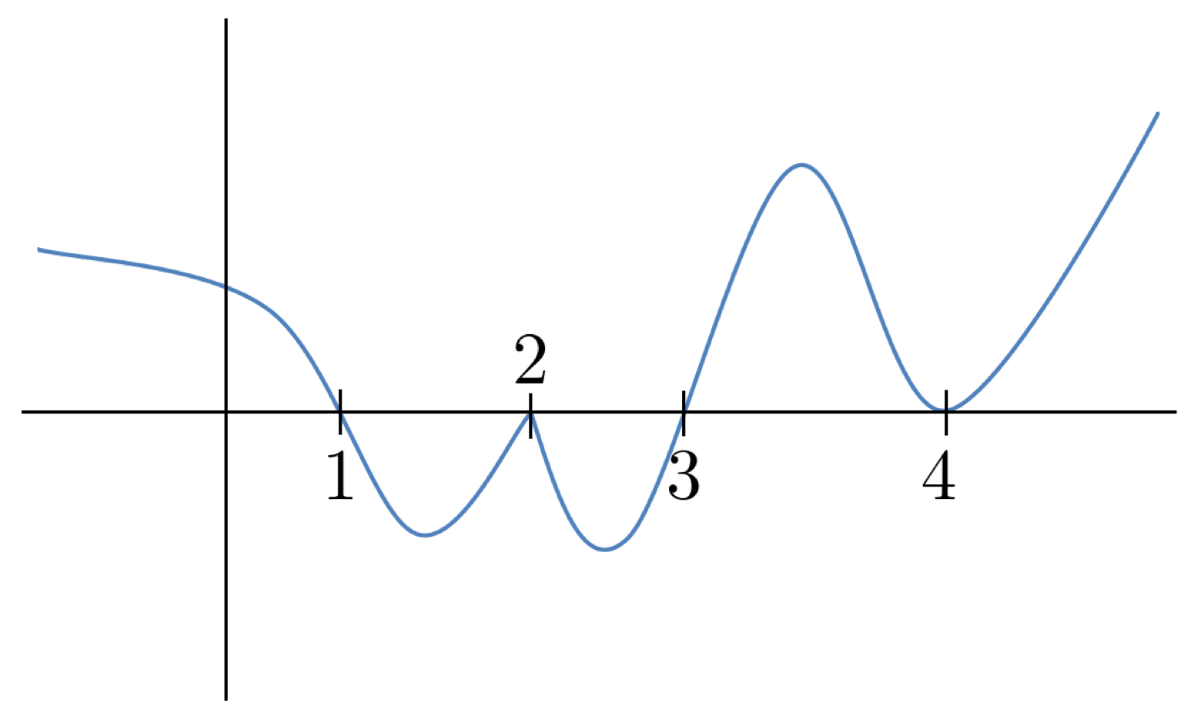
\includegraphics[width=0.5\textwidth]{ejer-a}
    \item Gr\'afica de la derivada de $f$.\\
        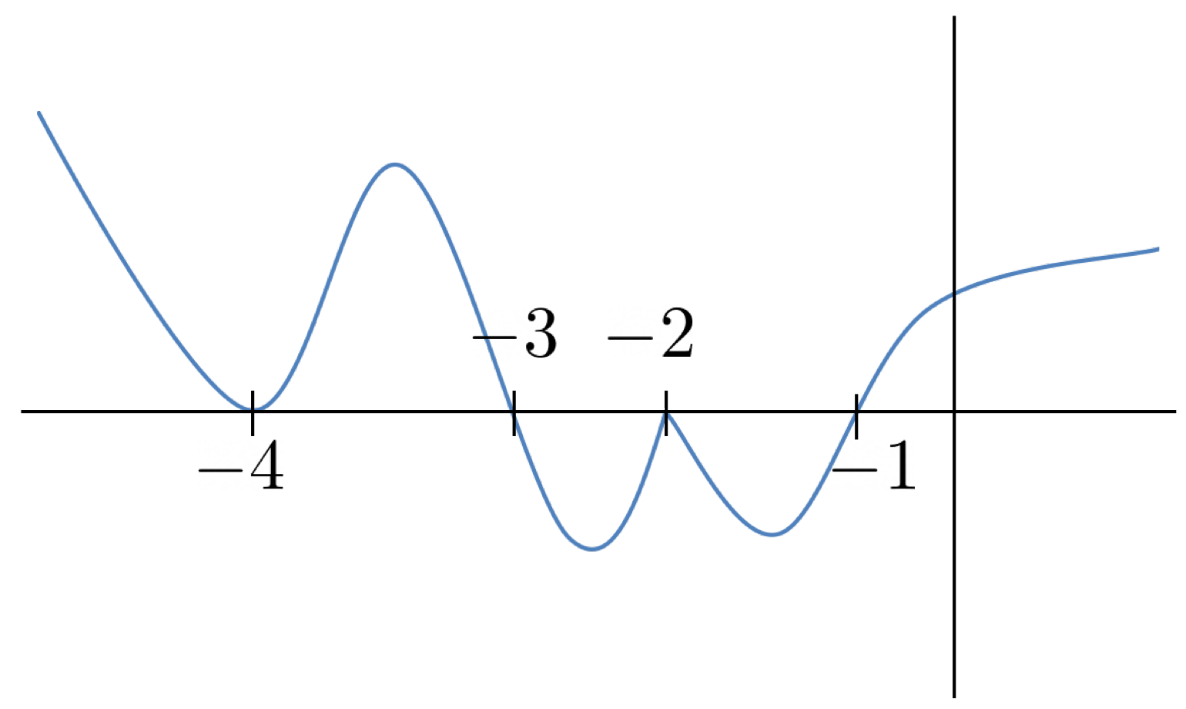
\includegraphics[width=0.5\textwidth]{ejer-b}
    \item Gr\'afica de la derivada de $f$.\\
        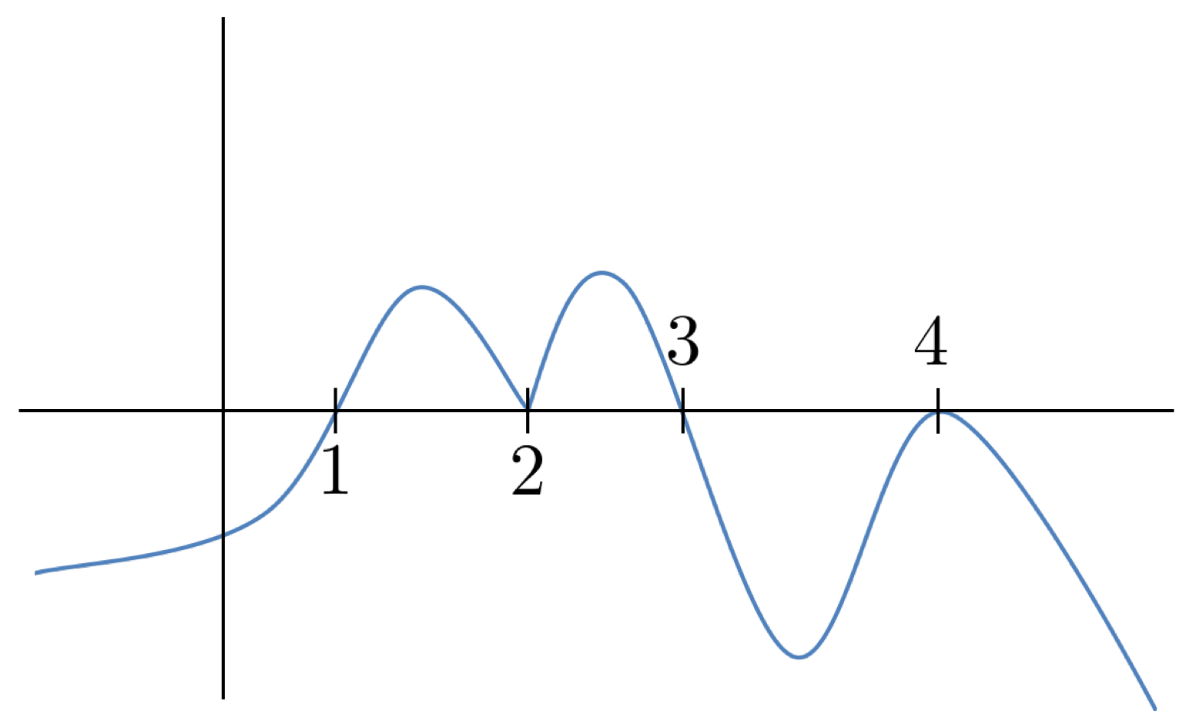
\includegraphics[width=0.5\textwidth]{ejer-c}
    \item Gr\'afica de la derivada de $f$.\\
        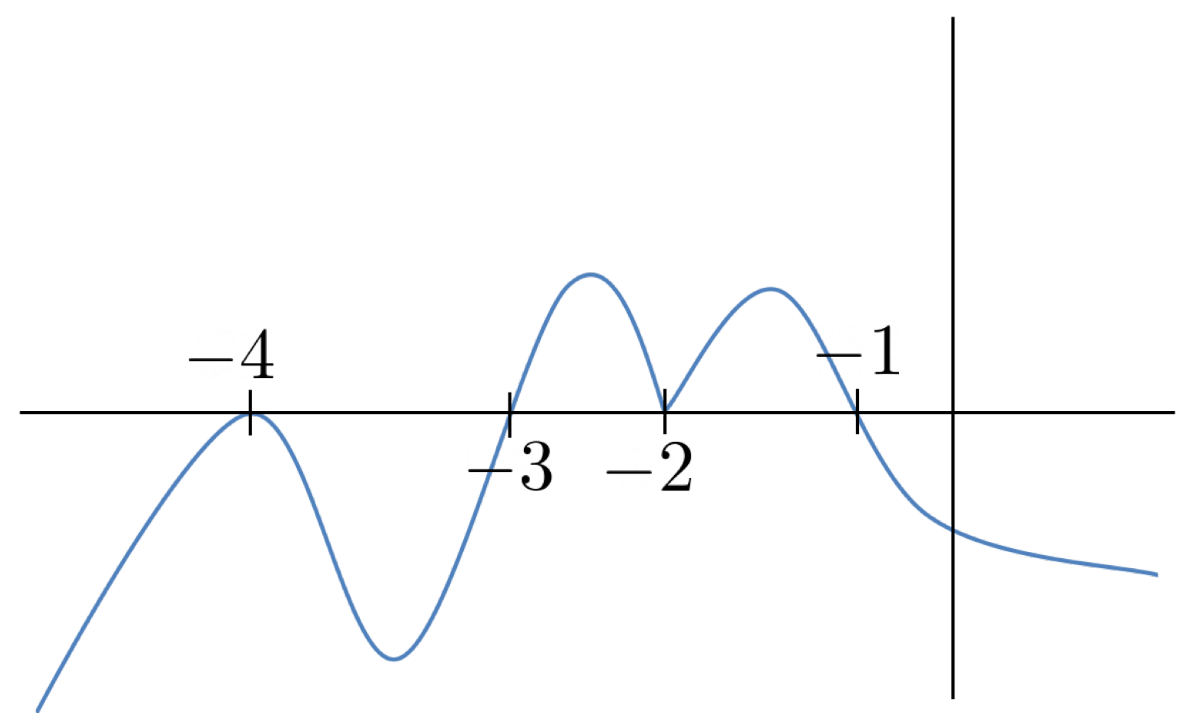
\includegraphics[width=0.5\textwidth]{ejer-d}
\end{enumerate}

%EJERCICIO 16 ----------------------------------------------------------------------------------
16. Utiliza los resultados sobre el significado de la derivada para esbozar la gr\'afica de las siguientes funciones (aplicar criterios de la primera y la segunda derivada).

\begin{enumerate}[\hspace{9px} a)]
    \item \(f(x)=x+\displaystyle\frac{1}{x}\)
    \item \(f(x)=x+\displaystyle\frac{3}{x^2}\)
    \item \(f(x)=\displaystyle\frac{x^2}{x^2-1}\)
    \item \(f(x)=\displaystyle\frac{1}{x^2+1}\)
\end{enumerate}

%EJERCICIO 17 ----------------------------------------------------------------------------------
17. Mostrar que:

\begin{enumerate}[\hspace{9px} a)]
    \item La suma de un n\'umero real positivo y su rec\'iproco es por lo menos 2.\\ \\
      Podemos representar el enunciado con la siguiente funcion:
      \[f(x) = x+\displaystyle\frac{1}{x}\] 
      Y si podemos mostrar que el minimo de dicha funcion es 2, podemos afirmar que no existe numero para el cual la suma con su rec\'iproco es mayor o igual a 2, y podemos encontrar puntos criticos de una funcion usando su derivada.\\*
      Sabemos que \[\displaystyle\frac{d}{dx}(f(x)+g(x)) = \displaystyle\frac{d}{dx}f(x)+\displaystyle\frac{d}{dx}g(x)\]
      Por lo tanto la derivada es: 
      \[f'(x): \ = 1-\displaystyle\frac{1}{x^2}\]
      Y tendra uno o mas puntos criticos cuando sea igual a 0, asi que \[1-\displaystyle\frac{1}{x^2}=0\Rightarrow\displaystyle\frac{1}{x^2}=1\Rightarrow x^2 = 1 \Rightarrow x=1\]   
      Es necesario revisar si es un maximo o un minimo, para lo cual usaremos la segunda derivada, siendo esta: \[f''(x)=\displaystyle\frac{2}{x^3}\]
      Evaluamos el punto critico que encontramos \(f''(1)=\displaystyle\frac{2}{1^3}\Rightarrow f''(1)=2\Rightarrow 2>0\)\quad Por lo que es un minimo.
      Sabiendo que el punto critico es un minimo, evaluamos en la funcion para obtener el valor critico
      \[f(1)=1+\displaystyle\frac{1}{1}\Rightarrow f(1)=2\]
      El minimo valor que puede tener la suma de un numero y su reciproco es 2
    \item Entre todos los rect\'angulos de igual per\'imetro, el de mayor \'area es el cuadrado.\\ \\
    Sabiendo que el perimetro de un rectangulo es \(p=2b+2h\) y su area \(bh\)
    Podemos usar el perimetro tal que: \[p=2b+2h\Rightarrow p-2h=2b\Rightarrow \displaystyle\frac{p}{2}-h=b\]
    Y sustituyendo en la operacion de area tenemos que \(f(h)=(\displaystyle\frac{p}{2}-h)h\Rightarrow f(h)=\displaystyle\frac{ph}{2}-h^2\).
    Tenemos ahora el area en funcion de la altura de un rectangulo, usando la derivada podemos encontrar con que altura tiene area maxima el rectangulo. \\*Si observamos que \(\displaystyle\frac{p}{2}\)es una constante entonces la derivada de esa funcion es: 
    \[f'(h)=\displaystyle\frac{p}{2}-2h\]
    Igualamos la derivada a 0 para encontrar puntos criticos.
    \[f'(h)=\displaystyle\frac{p}{2}-2h=0\Rightarrow \displaystyle\frac{p}{2}=2h\Rightarrow \displaystyle\frac{p}{4}=h\]
    Esto implica que el area tiene un maximo o un minimo cuando todos los lados son iguales, solo resta determinar si es max o min con la segunda derivada.
    \[f''(h)=-2\]
    Y como \(-2<0\) el punto critico es un maximo. 
    \item Entre todos los rect\'angulos con la misma \'area, el cuadrado es el de per\'imetro m\'inimo.\\ \\
    Sabiendo que el perimetro de un rectangulo es \(p=2b+2h\) y su area \(bh\)
    Podemos usar el area tal que: \[a=bh\Rightarrow \displaystyle\frac{a}{h}=b\]
    Y sustituyendo en la operacion del perimetro tenemos que \[f(h)=2\displaystyle\frac{a}{h}+2h\Rightarrow f(h)=\displaystyle\frac{2a}{h}+2h\]
    Tenemos ahora el perimetro en funcion de la altura de un rectangulo, usando la derivada podemos encontrar con que altura tiene perimetro minimo el rectangulo. Si observamos que \(2a\)es una constante entonces la derivada de esa funcion es: 
    \[f'(h)=-\displaystyle\frac{2a}{h^2}+2\]
    Igualamos la derivada a 0 para encontrar puntos criticos.
    \[f'(h)=-\displaystyle\frac{2a}{h^2}+2=0\Rightarrow \displaystyle\frac{2a}{h^2}=2\Rightarrow 2a=2h^2\Rightarrow a=h^2\]
    Podemos observar que esa es la formula del area que solo es cierta si \(h=b\), asi que el rectangulo tiene un perimetro maximo o minimo cuando es un cuadrado, usamos la segunda derivada para determinar cual de los dos es.
    \[f''(h)=\displaystyle\frac{4a}{h^3}\]
    Como \(a\) y \(h\) no pueden ser negativos entonces \(\displaystyle\frac{4a}{h^3}>0\), por lo que es un valor minimo.
    \item Entre todos los rect\'angulos que pueden inscribirse en una circunferencia, el cuadrado es el de \'area m\'axima. \\ \\
    Tomemos un rect\'angulos cuya base sea \(2x\) y su altura \(2y\), inscrito en un circulo de radio \(r\)\\
    Obervemos que, se forma un triangulo rectangulo con catetos \(x\) , \(y\) e hipotenusa \(r\) de lo cual podemos concluir por el teorema de Pitagoras 
    \[r^2=x^2+y^2\Rightarrow r^2-x^2=y^2\Rightarrow \sqrt{r^2-x^2}=y\]
    Sabemos que el area de el rect\'angulo es \(4xy\).\quad Podemos sustitur con la observacion anterior
    \[f(r)=4x\sqrt{r^2-x^2}\]
    Esta es una funcion de area respecto a radio, asi que usaremos la derivada para saber cuando alcanza un maximo.\\
    La regla de la cadena dice que la derivada de \(g(f(x))\) es \(g'(f(x))f'(x)\).
    \[f'(x)=4\sqrt{r^2-x^2}+\displaystyle\frac{-2x}{2\sqrt{r^2-x^2}}4x\Rightarrow 4\sqrt{r^2-x^2}-\displaystyle\frac{4x^2}{\sqrt{r^2-x^2}}\]
    Igualamos a 0 para encontrar puntos criticos
    \[4\sqrt{r^2-x^2}-\displaystyle\frac{4x^2}{\sqrt{r^2-x^2}}=0\Rightarrow 4(r^2-x^2)=4x^2\Rightarrow r^2-x^2=x^2\Rightarrow r^2=2x^2\Rightarrow \displaystyle\frac{r^2}{2}=x^2\Rightarrow \displaystyle\frac{r}{\sqrt{2}}=x\] 
    Tenemos el valor de \(x\) para un punto critico, resta encontrar el valor de \(y\) para dicho valor
    \[y=\sqrt{r^2-x^2}\Rightarrow y=\sqrt{r^2-(\displaystyle\frac{r}{\sqrt{2}})^2}\Rightarrow y=\sqrt{r^2-\displaystyle\frac{r^2}{2}}\Rightarrow y=\sqrt{\displaystyle\frac{r^2}{2}}\Rightarrow y=\displaystyle\frac{r}{\sqrt{2}}\] 
    Podemos observar que \(x\) y \(y\) tienen el mismo valor, lo cual prueba que el rectangulo de mayor area inscrita en un circulo es un cuadrado.
    \item La raz\'on de variac\'on del volumen de una esfera respecto a su radio, es igual a su \'area.\\ \\
    La razon de variacion de una funcion es su derivada, por lo que: 
    \[f(r)=volumen \qquad \qquad f'(r)=area\]
    Y sabiendo que:
    \[Volumen Esfera=\displaystyle\frac{4\pi}{3}r^3\qquad \qquad Area Esfera=4\pi r^2\]
    Observemos que \(\displaystyle\frac{4\pi}{3}\)es una constante, por lo que sea la funcion
    \[f(r)=\displaystyle\frac{4\pi}{3}r^3\]
    Su derivada sera
    \[f'(r)=3\displaystyle\frac{4\pi}{3}r^2\Rightarrow 4\pi r^2\]
\end{enumerate}

%EJERCICIO 18 ----------------------------------------------------------------------------------
18. Encuentre el punto para el cual:

\begin{enumerate}[\hspace{9px} a)]
    \item La recta tangente a la par\'abola \(f(x)=x^2-7x+3\), es paralela a la recta \(5x+3y-3=0\) \\ \\
    Dos rectas son paralelas si y solo si sus pendientes son iguales. Para la pendiente de la recta la representamos de la forma \(g(a) = f'(a)(x-a)+f(a)\)
    \[5x+3y-3\Rightarrow 5x-3=-3y\Rightarrow -\displaystyle\frac{5}{3}-1=y\]
    En la cual \(-\displaystyle\frac{5}{3}\) es la pendiente\\ \\
    La derivada de una funcion es la pendiente de la recta tangente en un punto de la funcion por lo que si obtenemos la derivada y la igualamos a la pendiente encontrada podremos encontrar el punto en el cual es paralela a la recta dada.
    \[f(x)=x^2-7x+3\Rightarrow f'(x)=2x-7\Rightarrow 2x-7=-\displaystyle\frac{5}{3}\Rightarrow 3(2x-7)=-5\]
    \[\Rightarrow 6x-21=-5\Rightarrow 6x=16\Rightarrow x=\displaystyle\frac{8}{3}\]
     Ese es el punto en el cual la tangente y la recta son paralelas.
    \item La recta tangente a la par\'abola \(f(x)=x^2-7x+3\), es paralela a la recta \(3x-y-4=0\) \\ \\
    Dos rectas son paralelas si y solo si sus pendientes son iguales. Para la pendiente de la recta la representamos de la forma \(g(a) = f'(a)(x-a)+f(a)\)
    \[3x-y-4\Rightarrow 3x-4=y\]
    En la cual \(3\) es la pendiente\\ \\
    La derivada de una funcion es la pendiente de la recta tangente en un punto de la funcion por lo que si obtenemos la derivada y la igualamos a la pendiente encontrada podremos encontrar el punto en el cual es paralela a la recta dada.
    \[f(x)=x^2-7x+3\Rightarrow f'(x)=2x-7\Rightarrow 2x-7=3\Rightarrow 2x=10\Rightarrow x=5\]
     Ese es el punto en el cual la tangente y la recta son paralelas.
    \item La recta tangente a la pa\'rabola \(f(x)=x^2-7x+3\), es paralela a la recta \(2x+3y-3=0\) \\ \\
    Dos rectas son paralelas si y solo si sus pendientes son iguales. Para la pendiente de la recta la representamos de la forma \(g(a) = f'(a)(x-a)+f(a)\)
    \[2x+3y-3\Rightarrow 2x-3=-3y\Rightarrow -\displaystyle\frac{2}{3}-1=y\]
    En la cual \(-\displaystyle\frac{2}{3}\) es la pendiente\\ \\
    La derivada de una funcion es la pendiente de la recta tangente en un punto de la funcion por lo que si obtenemos la derivada y la igualamos a la pendiente encontrada podremos encontrar el punto en el cual es paralela a la recta dada.
    \[f(x)=x^2-7x+3\Rightarrow f'(x)=2x-7\Rightarrow 2x-7=-\displaystyle\frac{2}{3}\Rightarrow 3(2x-7)=-2\]
    \[\Rightarrow 6x-21=-2\Rightarrow 6x=19\Rightarrow x=\displaystyle\frac{19}{6}\]
     Ese es el punto en el cual la tangente y la recta son paralelas.
\end{enumerate}

\vfill

\textbf{F\'ormula cuadratica:}
\begin{proof}
\begin{align*}
    ax^2+bx+c&=0\\
    (4a)(ax^2+bx+c)&=0(4a) \quad &&\text{Por el teorema $a=b \iff ac=bc$.}\\
    (4a)(ax^2+bx+c)&=0 &&\text{Por el teorema $0a=0$.}\\
    (4a)(ax^2)+(4a)(bx)+(4a)(c)&=0 &&\text{Por el axioma de la distributividad.}\\
    4a^2x^2+4abx+4ac&=0 &&\text{Operando.}\\
    4a^2x^2+4abx+4ac-4ac+b^2&=0+b^2-4ac &&\text{Por el teorema $a=b \iff a+c=b+c$.}\\
    4a^2x^2+4abx+0+b^2&=0+b^2-4ac &&\text{Por el axioma del inverso de la suma.}\\
    4a^2x^2+4abx+b^2&=b^2-4ac &&\text{Por el axioma del neutro de la suma.}\\
    (2ax+b)^2&=b^2-4ac &&\text{Por el teorema $(a+b)^2=a^2+2ab+b^2$.}\\
    2ax+b&=\pm \sqrt{b^2-4ac} &&\text{Sacando raiz cuadrada a ambos lados.}\\
    2ax+b-b&=-b \pm \sqrt{b^2-4ac} &&\text{Por el teorema $a=b \iff a+c=b+c$.}\\
    2ax+0&=-b \pm \sqrt{b^2-4ac} &&\text{Por el axioma del inverso de la suma.}\\
    2ax&=-b \pm \sqrt{b^2-4ac} &&\text{Por el axioma del neutro de la suma.}\\
    \frac{2ax}{2a}&=\frac{-b\pm \sqrt{b^2-4ac}}{2a} &&\text{Por el teorema $a=b \iff ac=bc$.}\\
    1x&=\frac{-b\pm \sqrt{b^2-4ac}}{2a} &&\text{Por el axioma del inverso de la multiplicación.}\\
    x&=\frac{-b\pm \sqrt{b^2-4ac}}{2a} &&\text{Por el axioma del neutro de la multiplicación.}
\end{align*}
\end{proof}

\end{document}
